Tracking \footnote{Tracking,http://www.bmva.org/bmvc/2014/files/paper038.pdf} คือระบบที่ใช้สำหรับการติดตามการเคลื่อนไหวของวัตถุที่สนใจที่อยู่ในรูปภาพ นำมาใช้ในการแก้ปัญหาด้านการคำนวณของคอมพิวเตอร์ ทำให้โปรแกรมสามารถงานได้เร็วมากขึ้น

\begin{figure}[!ht]
	\centering
	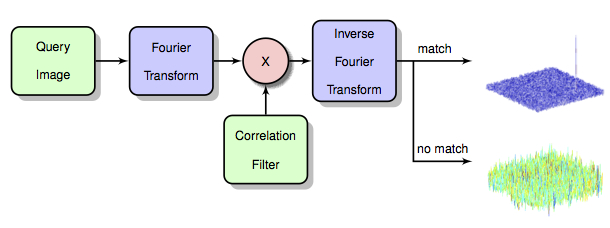
\includegraphics[width=1\textwidth]{chapter2/images/track-concept.png}
		\caption{Track concept}
    	\label{fig:Track concept}
\end{figure}

จากภาพ \ref{fig:Track concept} จะเป็นหลักการในการทำนายตำแหน่งต่อไป เริ่มจากการนำภาพมาแปลงให้อยู่ในรูปของฟูรีเย (fourier transform) และนำมาคูณกับ correlation filter ซึ่งเป็นฟิลเตอร์ที่ใช้สำหรับการหาความสัมพันธ์กับวัตถุในภาพ ต่อมาทำการอินเวอร์สฟูริเย (inverse fourier transform) เพื่อตรวจสอบว่าวัตถุในภาพนั้นอยู่ที่ตำแหน่งใด โดยมีการคำนวณเริ่มจากหา correlation filter ที่ดีที่สุดโดยใช้วิธี minimizing the sum of square errors ดังนี้
\\
\centerline{$\epsilon = \left \| \sum_{l = 1}^{d} h^{l} \star f^{l} - g \right \| + \lambda \sum_{l = 1}^{d} h^{l}\left \| h^{l} \right \|^2$}		\\
\centerline{$\epsilon$ คือ ค่าความคลาดเคลื่อน}							\\
\centerline{$d$ คือ จำนวนมิติของ feature map ของภาพ}						\\
\centerline{$h$ คือ correlation filter}									\\
\centerline{$f$ คือ พื้นที่สี่เหลี่ยมของวัตถุที่สนใจที่ได้จากการทำ feature map}			\\
\centerline{$g$ คือ ผลลัพธ์ correlation ที่ต้องการของ $f$}					\\
\centerline{$\lambda$ คือ regularization term}							\\
เมื่อพิจารณาจากรูปภาพเดียวในกรณที่เวลา(t) เท่ากับ 1 จะสามารถจัดรูปสมการด้านบนได้ดังนี้ 
\\
\centerline{$H^{l} = \frac{\bar{G}F^{l}}{\sum_{k=1}^{d}\bar{F^{k}}F^{k} + \lambda}$}		\\
\\
\centerline{$H_{t}^{l} = \frac{A_{t}^{l}}{B_{t}}$}									\\
\\
\centerline{$A_{t}^{l} = (1-\eta )A_{t-1}^{l} + \eta \bar{G_{t}}F_{t}^{l}$}					\\
\\
\centerline{$B_{t} = (1-\eta )B_{t-1} + \eta \sum_{k=1}^{d}\bar{F_{t}^{k}}F_{t}^{k}$}		\\
\centerline{$H$ คือ correlation filter}								\\
\centerline{$\eta$ คือ อัตราการเรียนรู้}												\\
\centerline{$\bar{G}$ คือ $g$ ที่ทำการทำ complex conjugation}								\\
\centerline{$F$ คือ พื้นที่สี่เหลี่ยมของวัตถุที่สนใจที่ได้จากการทำ feature map}						\\
\centerline{$\bar{F}$ คือ $f$ ที่ทำการทำ complex conjugation}								\\
\centerline{$t$ คือ เวลา}														\\
จากสมการที่ได้มาจะสามารถทำให้หาตำแหน่งต่อไปของวัตถุที่สนใจจากสมการต่อไปนี้
\\
\centerline{$y = F^{-1}\left \{ \frac{\sum_{l = 1}^{d} \bar{A^{l}}Z^{l}}{B + \lambda} \right \}$}		\\
\centerline{$y$ คือ correlation score}													\\
\centerline{$F^{-1}$ คือ การทำ inverse discrete fourier transform}								\\
\centerline{$Z$ คือ พื้นที่สี่เหลี่ยมของวัตถุที่สนใจที่ได้จากการ feature map ของภาพใหม่}				\\
โดยค่าของ $y$ ที่ได้ออกมาจะทำให้รู้ถึงตำแหน่งของวัตถุที่สนใจได้ ณ ตำแหน่งที่ $y$ มีค่าสูงสุด